In this chapter I am going to introduce the package provided by Salesforce called Foundation. This package offers the possibility to create simulations with multiple agents that interacts in a 2D world. First a presentation of the the Gather and Trade simulation setup will be purposed, followed by a description of the agents involved, their action set, observation and scope.

\textcolor{red}{descrivi il capitolo quando lo hai finito}

\section{Gather and trade}

The simulation that will be used throght the dissertation is called gather and trade. This simulation takes place in a 2D map that represent the world where the agents lives and interact. The shape of the world is a 25x25 grid where are disposed various kinds of entities. Within this world 4 agents are free to move around, gather resources, trade them and use them to build houses. These agents are different for their skill level, allowing them to have higher/lower rewards for their actions. A fifth agent, called policy maker, is asked to tax and redistribute the income of the 4 previous agents, based on informations about their endowments, but not their skill.

\subsection{World and entities}

As said before the map is a 25x25 grid that where are present some entities. Some of these are visible in the world, others are just present in the agents endowment.

\begin{itemize}
    \item Water
    \item House
    \item Source Block (Wood and Stone)
    \item Wood and Stone
    \item Coins
    \item Labor
\end{itemize}


Water is a simple world block that has no use other than avoiding agents to pass through. We can see from Figure \ref{img:map_0} that the water is used to divide the world in 4 macro areas, each one with different resources. 
A House is a block that is not present at the beginning of the simulation, but it can be built by agents in any empty block, agents can't walk through houses either.

Sorce blocks are two entities that spawns stochastically resources, namely wood and stone, as we can see from Figure \ref{img:map_0} in the four areas divided by water we have a zone with both wood and stone source block, two other areas with just one kind of source block and the last one that is empty. 

Coins is the measurement of the value produced in the world. Coins are generated when a house is built, the agent that builds the house is rewarded with a certain amount of coins that variates with the skill level.

Labor is a measurement of the total effort exherted by an agent, this is generated every time an agent takes an actions and generates disutility.


\begin{figure}[h!]
    \centering
    \linespread{.9} 
    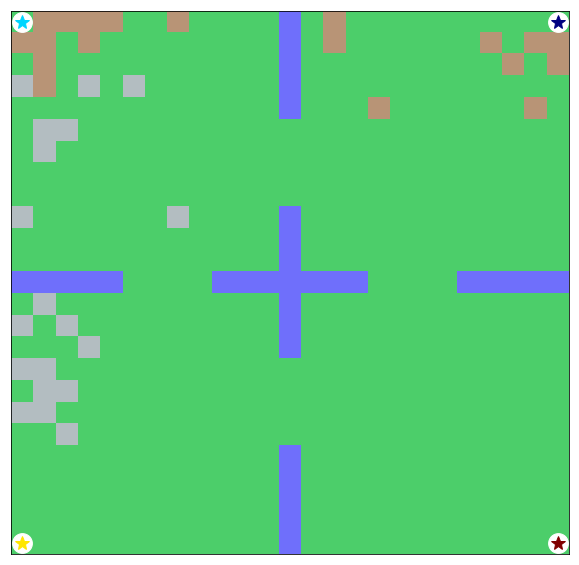
\includegraphics[width=0.5\textwidth]{Resources/imgs/Map_0.png}
    \caption[Rendering of the world at inital conditions: ]%
    {\label{img:map_0}Rendering of the world at inital conditions: \small \textit{this is a rendering of the world map at the first timestep of the simulation, blue block are water, brown blocks are wood source, grey block are Stone source. The four corners are the starting positions for the 4 agents.}}
\end{figure}



\subsection{Game dynamics}

A problem that has a continuous flow of agent-environment interactons can be formalized by a Finite Markov Decision problem \cite{sutton2018reinforcement}. In particular this simulation is a partial-observable multi-agent Markov Games (MGs). The problem is defined by the tuple \(\left(  S,A,R, \text{\textcolor{red}{simbolo}} ,\gamma, o, \mathcal{T} \right) \) where \( S \) is the state space and \( A \) is the action space. 

The simulation is composed by a series of episodes, each of length \( H \) timesteps. At every point in time \( t \in [0,H] \) the episode is characterized by a state \( s_t \), representing the current world environment, every agent performs an action \( a_{i,t}  \)  given the current partial observation \( o_{i,t}\) of the world state, and recives a reward \( r_{it}  \). Afterwards the environment transits to a new state \( s_{t+1} \) according to the transition distribution \(  \mathcal{T}(s_{t+1}|s_t,\boldsymbol{a}_t)\). This chain of interactions state-action-reward/state carries on until the end of an episode.

\begin{equation*}
     s_0 \,  \rightarrow_{\boldsymbol{o}_0}\, \boldsymbol{a}_0 \,\rightarrow\, r_1 , s_1 \,\rightarrow_{\boldsymbol{o}_1}\, \boldsymbol{a}_1 \,\rightarrow ... \rightarrow_{\boldsymbol{o}_{H-1}}\, \boldsymbol{a}_{H-1} \,\rightarrow\, r_H , s_H
\end{equation*}

Here \( \boldsymbol{a} \) and \( \boldsymbol{o} \) are the vectorized observations and actions for all the five agents. Given the particular structure of the simulation every single agent will recive an observation at every timestep (different for everyone, more on that later), but only at the 4 basic agents will be asked to perform an action, the policy maker will act only upon a certain condition met. In this case the episode last for 1000 timestep and the policy maker is asked to act (tax the other agents) every other 100 steps. The existence of multiple episodes is necessary for the 4 agents and the policy maker to define their own optimal policy \( \pi_i(o_{i,t}, h_{i,t-1};\theta_i^*) \), this optimization process will be the focus of chapter \textcolor{red}{RL}.

\subsection{Agents}

From what above we know that the four basic agents are endowed with labor, coins, wood and stone. They live in the world map, can act within it and their objective is to maximize their $\gamma$-discounted utility function. Now I will describe in more in detail the agents starting from the inforamtions that they receive at each timestep, then talking about the actions that they are allowed to take and finally about their objective. 

\paragraph{Observation space:} Given that this simulation is a partial-observable multi-agent Markov Game, the observation that agent \( i \) receive at time \( t \) is not complete but partial, this inforamtions can be summarized in the following way:

\begin{itemize}
    \item \(o_{i,t}^{\text{world state}}\): world map situation surrounding the agent, this is limited to the 11x11 grid around the agent \( i \).
    \item \(o_{i,t}^{\text{market state}}\): full information about the market state for wood, stone and available trades.
    \item \(o_{i,t}^{\text{agent}}\): public resouces and coin endowments (this information is also available to the policy maker) and private labor performed and skill level.
    \item \( o_{i,t}^{\text{tax}} \): tax structure
    \item \( o_{i,t}^{\text{other}} \): other inforamtions (ex. action mask)
\end{itemize}
 
the full observation space can be seen in Table \ref{tab:full_obs}

\paragraph{Action space:} The agent can take one action per timestep and can choose this action from the 50 listed below:

\begin{itemize}
    \item \textbf{Movement}: 4 actions for the basic movements N, S, E, W
    \item \textbf{Gather}: 1 action for gahtering
    \item \textbf{Trade}: 44 actions for trading resouces
    \item \textbf{Idle}: 1 action that do notthing
\end{itemize}

The movements actions along with gather do not need much of an explaination, these are simple actions that costs a quantity of 0.21 labor units each time pursued. The building action require the agent to consume (destroy) one unit of wood and one unit of Stone, as a consequence he gains 2.1 units of labor and an amount of coin that depends on his skill level. The most complicate set of actions are the one that rules trading. Each one of them is a combination of the 11 price levels [0,1,...,10] that the agent is willing to (pay/request) for each side (bid/ask) and for each resource (wood/stone). A trading open action remains open for 50 tunrs, if in this time span it is matched by the corresponding counter action at the same price (a bid for an ask and vice versa) then the trade takes place and each agent gets a 0.05 units of labor.

The action mask, present in the observation space, is a touple of binary values of length 50 that "masks" inconclusive actions, such as moving north while at the north border of the map, or building a house without the required wood and stone. This is used in the learning process to avoid wasting time in exploring meaningless actions.

\paragraph{Agent objective}

Agents in the simulation earn coins when building houses or trading goods, 

The utility for the four agents is an isoelastic utility:

\begin{equation}
u_i(x_{i,t}, l_{i,t}) = crra(x_{i,t}^c) - \vartheta_k l_{i,t}\,, \quad crra(z) = \frac{z^{1- \eta}-1}{1-\eta}\,,\,\, \eta > 0
\end{equation}

Where \( l_{i,t} \) is the cumulative labor associated with the actions taken up to time \( t \), \( x_{i,t}^c \) is the coin endowment and \( \vartheta \) is a function utilized for labor anihilation with the following specification \( \vartheta_k = 1- exp\left(- \frac{\textit{episode completitions}}{\textit{energy warmup constant (k)}}\right)\). This variable will play an important role during the two step optimization process purposed in the original paper. In particular during the phase 1 of training the labor cost is annihilated to help agents avoid sub-optimal behaviours. And \( \eta \) determies the degree of nonlinearity of the utility. This utility function is assumed to be the same for all the agents.

The maximization problem is solved for a rational behaving agent by optimizing the total discounted utility over time,

\begin{equation}
\forall i \,:\, \max_{\pi_i}\mathbb{E}_{a_i \sim \pi_i, \boldsymbol{a}_{-i} \sim \boldsymbol{\pi}_{-i}, s^{'}\sim\mathcal{T}}\left[ \sum_{t=1}^H \gamma^t r_{i,t} + u_i({x_{i,0}l_{i,0}})\right]
\label{eq:agent_max}
\end{equation}


with \( r_{i,t} = u_i(x_{i,t},l_{i,t})  - u_i(x_{i,t-1},l_{i,t-1}) \) being the istantaneous reward of agent \( i \) at time \( t \). Equation \ref{eq:agent_max} illustrates a multi-agent optimization problem in which actors optimize their behavior at the same time, since the utility of each agent is dependent on the behavior of other agents. Another agent, for example, may deny an agent access to resources, limiting how many houses the agent can create in the future and hence its utility. While computing equilibria for complicated environments like this is still out of reach, we will see in \textcolor{red}{RL chapter} how RL may be utilized to produce meaningful, emergent behaviors.


\subsection{Policy maker}

The policy maker, or social planner, differs deeply from the previous agents. Being the focus of the research question it's structure and behavior changes a lot in every single simulaion. 

\paragraph{Observation space:} The observation space of the social planner depends on the simulation, for most of the simulations no observation is needed. 

\textcolor{red}{se riesci a fare RL anche su di lui descrivi l'obs space di quella simulazione}

\paragraph{Action space:} the action space is quite similar amongs all the simulations, the social planner has to decide how much to tax the individuals according to their total income. If the policy maker is 

\textcolor{red}{non è facile finchè non ho deciso le simulazioni da fare ... magari lo rimado a dopo}


